\documentclass[11pt,a4paper]{article}
\usepackage[T1]{fontenc}
\usepackage[utf8]{inputenc}
\usepackage{amsmath,amsthm}
\usepackage{newpxtext,newpxmath}
\usepackage[margin=26mm,headheight=15pt]{geometry}
\usepackage{microtype,mathtools,amsthm,booktabs,longtable,array,graphicx,xcolor}
\usepackage{enumitem,fancyhdr,xurl,hyperref,cleveref}
\hypersetup{colorlinks=true,linkcolor=blue!45!black,citecolor=blue!45!black,urlcolor=blue!45!black,
 pdftitle={Beyond Polynomial Diagonals: Bayesian Operators for Fabius--Rvachev Laws},
 pdfauthor={Research article prepared for Vladimir Reshetnikov}}
\pagestyle{fancy}\fancyhf{}
\fancyhead[L]{\small Fabius--Rvachev Bayesian operators}
\fancyhead[R]{\small Research article}
\fancyfoot[L]{\small 29 September 2026}\fancyfoot[R]{\thepage}
\setlength{\parskip}{4pt}\setlength{\parindent}{1.2em}
\setlist{nosep,leftmargin=*}
\numberwithin{equation}{section}
\newtheorem{theorem}{Theorem}[section]
\newtheorem{lemma}[theorem]{Lemma}
\newtheorem{proposition}[theorem]{Proposition}
\newtheorem{corollary}[theorem]{Corollary}
\theoremstyle{definition}\newtheorem{definition}[theorem]{Definition}
\newtheorem{problem}[theorem]{Research question}
\theoremstyle{remark}\newtheorem{remark}[theorem]{Remark}
% ed. (2026-09-29): unnumbered environment for editorial notes.
\newtheorem*{ednote}{Editorial note (ProveIt, 2026-09-29)}
\newcommand{\R}{\mathbb R}\newcommand{\C}{\mathbb C}
\newcommand{\E}{\mathbb E}\newcommand{\Pp}{\mathbb P}
\newcommand{\Var}{\operatorname{Var}}\newcommand{\Cov}{\operatorname{Cov}}
\newcommand{\supp}{\operatorname{supp}}\newcommand{\rank}{\operatorname{rank}}
\newcommand{\sinc}{\operatorname{sinc}}\newcommand{\HS}{\mathrm{HS}}
\newcommand{\dd}{\,\mathrm d}\newcommand{\ii}{\mathrm i}
\newcommand{\calC}{\mathcal C_m}\newcommand{\calP}{\mathcal P}
\newcommand{\ip}[2]{\langle #1,#2\rangle}
\newcommand{\norm}[1]{\lVert #1\rVert}
\newcommand{\repo}{\texttt{ProveIt}}
\title{\LARGE\bfseries Beyond Polynomial Diagonals\\[5pt]
\Large Nuclear Bayesian Operators, Exact Null Modes,\\
and a R\'enyi Phase Transition for Fabius--Rvachev Laws}
\author{Research article prepared for Vladimir Reshetnikov}
\date{29 September 2026}
\begin{document}
\maketitle
\begin{abstract}
We study the conditional-expectation operator associated with a finite prefix of a geometric sum of independent uniform random variables. The motivating repository asks for its Appell/Legendre singular system and its R\'enyi information. We prove that the operator belongs to every Schatten class and that its nonzero singular values satisfy a quantitative log-normal upper bound. At the same time, it has an infinite-dimensional kernel containing explicit exponential-polynomial modes. Every polynomial restriction is algebraically unipotent and invertible, but its Hilbert-space condition number grows at least factorially. Thus polynomial triangularity is not a singular-value decomposition.

We give exact moment-determinant and exterior-power formulas, a low-degree obstruction to cyclotomic $q$-product formulas, and a Gaussian rigidity theorem for linear reverse regression. For the geometric-uniform law, a cubic statistic strictly improves the linear correlation bound. We also prove that every finite R\'enyi order is finite at every finite depth, whereas the limiting excess above the Shannon information changes behavior exactly at order two: it has an explicit finite limit for $1<\alpha\le2$ and diverges for $\alpha>2$. Finally, no deterministic or randomized postprocessing of the original prefix can be rate-distortion optimal at its exact mean-square error. All principal claims are proved in the text; exact-arithmetic checks and high-precision finite-dimensional diagnostics accompany the article. No Lean verification or literature-wide priority is claimed.
\end{abstract}
\newpage
\tableofcontents
\newpage

\section{Research target and scope}
\label{sec:scope}
The geometric convolution behind the Fabius--Rvachev function is particularly well suited to studying the difference between algebraic identities and statistical information. A finite prefix determines many exact polynomial formulas, but conditional expectation is an operator between two \emph{different weighted Hilbert spaces}. Its singular values depend on those weights, not just on the diagonal of a coefficient matrix.

The information-frontier report in \repo\ \cite{frontier,repo} poses three directly relevant questions, with source labels \texttt{prob:Bayesian-spectrum}, \texttt{prob:TM-Renyi}, and \texttt{prob:exact-RD}. The first asks for polynomial triangularization, singular values, determinants, and possible $q$-product formulas. The second asks for R\'enyi information, particularly the collision order $\alpha=2$. The third asks, in part, whether an optimal reproduction can be obtained by correcting a geometric prefix. The report also suggests an Appell diagonal involving $q^{mn}$. For the operator actually defined there, the leading polynomial coefficient is instead one.

This article provides structural answers rather than an unsupported closed formula for every singular value. Its main advances within the inspected material are the all-Schatten theorem with an explicit decay exponent, the coexistence of exact null modes and factorially ill-conditioned polynomial inverses, and the finite-depth/large-depth R\'enyi distinction. The corrected-prefix question has a complete negative answer at the stated distortion. The full rate-distortion expansion and a closed formula for the nonzero singular spectrum remain separate questions.

\subsection{What is classical, and what is established here}
The Appell convolution identity is classical; it is closely related to the martingale identities discussed by Anshelevich \cite{anshelevich}. Gram determinants, conditional expectation as an $L^2$ contraction, Jacobi approximation, and maximal correlation are also established tools \cite{dlmf,xu,anantharam}. We provide their needed specializations and proofs, and do not present these tools as discoveries. The work here is their combination with the precise geometric-uniform channel, together with the resulting operator estimates, obstructions, and limiting information theorem.

The source report already gives $I(X_q;S_{q,m})=m\log(1/q)$ and describes the limiting centered information density for transform parameters inside $(-1,1)$ \cite{frontier}. Our R\'enyi theorem proves convergence of the relevant exponential moments up to the positive boundary, identifies that boundary exactly, and proves divergence beyond it. Merely knowing convergence in distribution of information densities would not establish these conclusions.

\subsection{Conventions}
All logarithms are natural. The R\'enyi information used here is
\[
 I_\alpha(S;X)=D_\alpha(P_{S,X}\Vert P_S\otimes P_X),
\]
not Sibson or Arimoto information. The distinction is essential. We use the standard divergence conventions of \cite{renyi}. A Schatten class $\mathcal S_p$, for any $p>0$, consists of compact operators whose singular values have summable $p$th powers. For $p<1$ the associated expression is a quasi-norm, not a norm. Operators may act between different Hilbert spaces; traces below are taken only for genuine endomorphisms such as $\calC^*\calC$.

\section{The geometric-uniform channel}
\label{sec:channel}
Let $U_0,U_1,\ldots$ be independent and uniform on $[-1,1]$, and fix $0<q<1$. Put
\begin{align}
 X=X_q&=(1-q)\sum_{j\ge0}q^jU_j,\label{eq:X}\\
 S=S_{q,m}&=(1-q)\sum_{j=0}^{m-1}q^jU_j,\qquad r=q^m,\quad a=1-r,
 \label{eq:S}\\
 T&=rX',\qquad X=S+T,\label{eq:decomp}
\end{align}
where $X'$ is independent of $S$ and has the same distribution as $X$. Denote the densities of $X,S,T$ by $f,b,p$, respectively. Then
\begin{equation}
 p(y)=r^{-1}f(y/r),\qquad f=b*p,
 \qquad \supp f=[-1,1],\quad \supp b=[-a,a].
 \label{eq:densities}
\end{equation}
The variance and characteristic function are
\begin{equation}
 V=\Var X=\frac{1-q}{3(1+q)},\qquad
 \phi_X(t)=\prod_{j\ge0}\sinc\bigl((1-q)q^jt\bigr),
 \quad \sinc u=\frac{\sin u}{u}.
 \label{eq:variance-product}
\end{equation}
At $q=1/2$, $f$ is the probability-normalized Rvachev up-function on $[-1,1]$; the classical probability and Fourier descriptions are discussed in \cite{arias}.

\begin{lemma}[Regularity and prefix geometry]
\label{lem:regularity}
The density $f$ is $C^\infty(\R)$, is positive on $(-1,1)$, and is flat at both endpoints. Moreover,
\begin{equation}
 \norm{f}_\infty\le \frac1{2(1-q)}.
 \label{eq:fmax}
\end{equation}
For each fixed $q,m$, there are positive constants $c_-,c_+$ such that
\begin{equation}
 c_-(a^2-s^2)^{m-1}\le b(s)\le c_+(a^2-s^2)^{m-1},\qquad |s|<a.
 \label{eq:prefix-comparison}
\end{equation}
In particular, for some $d>0$,
\begin{equation}
 \Pp\{|S-s|\le h\}\ge d h^m
 \quad (|s|\le a,\ 0<h\le a).
 \label{eq:smallball}
\end{equation}
Finally, as $m\to\infty$ with $q$ fixed, $b_m\to f$ uniformly on $\R$.
\end{lemma}
\begin{proof}
The convolution of $N$ uniform densities is a compactly supported spline of class at least $C^{N-2}$. Convolving with the remaining probability measure preserves this regularity. Taking $N$ arbitrarily large proves smoothness of $f$ on the entire real line and therefore flatness at the support endpoints. Positivity follows by taking a sufficiently long finite prefix whose support contains a given interior point, and integrating its positive density against a suitable part of the tail. The first uniform factor has density bounded by $1/[2(1-q)]$, proving \eqref{eq:fmax}.

Write $w_j=(1-q)q^j$. Near the upper endpoint the density of the prefix is exactly
\begin{equation}
 b(a-u)=\frac{u^{m-1}}{(m-1)!\prod_{j=0}^{m-1}(2w_j)},
 \qquad 0<u<2\min_{j<m}w_j.
 \label{eq:prefix-edge}
\end{equation}
This is the elementary simplex-volume formula for the deficits of the uniforms. The same formula holds at the lower endpoint. On compact subintervals of $(-a,a)$ the density is positive and continuous when $m\ge2$; when $m=1$ it is constant. The quotient in \eqref{eq:prefix-comparison} thus has positive finite endpoint limits and is bounded above and below. Integrating that comparison over a one-sided interval of length comparable to $h$ proves \eqref{eq:smallball}.

For uniform convergence, fix the density $g$ of the first two factors. It is globally Lipschitz, with a finite constant $L_q$. For $m\ge2$, $b_m=g*\nu_m$ for a probability measure $\nu_m$, hence $b_m$ is also $L_q$-Lipschitz. Since $f=b_m*p$ and $|T|\le r$,
\[
 \norm{b_m-f}_\infty\le L_qr\longrightarrow0.
\]
\end{proof}

The operator and its adjoint are
\begin{align}
 \calC &:L^2(f(x)\dd x)\longrightarrow L^2(b(s)\dd s),
 & (\calC g)(s)&=\int g(s+y)p(y)\dd y,\label{eq:C}\\
 (\calC^*h)(x)&=\frac{\int h(s)b(s)p(x-s)\dd s}{f(x)},
 && |x|<1.\label{eq:adjoint}
\end{align}
The kernel relative to these two probability measures is
\begin{equation}
 K(s,x)=\frac{p(x-s)}{f(x)}.
 \label{eq:kernel}
\end{equation}
Values at the endpoints, where $f=0$, do not affect the operator. Both operators preserve constants and are contractions. We allow complex-valued functions when describing Fourier modes; complexification does not change the singular values of the real operator.

\section{The main spectral theorem}
\label{sec:main-spectral}
\begin{theorem}[Nuclearity, null modes, and spectral decay]
\label{thm:spectral}
Fix $0<q<1$ and an integer $m\ge1$. The operator \eqref{eq:C} has dense range and an infinite-dimensional kernel. Its positive singular values form an infinite sequence
\[
 1=s_1(\calC)>s_2(\calC)\ge s_3(\calC)\ge\cdots>0
\]
converging to zero; the singular value $1$ is simple. For every $p_0>0$, $\calC\in\mathcal S_{p_0}$, and more precisely
\begin{equation}
 \limsup_{n\to\infty}
 \frac{\log s_n(\calC)}{(\log n)^2}
 \le-\frac1{6\log(1/q)}.
 \label{eq:lognormal-spectrum}
\end{equation}
The constant in this bound is not asserted to be optimal. It is a fixed-$q$, fixed-$m$ statement, not a bound uniform as $q\to1$ or $m\to\infty$.
\end{theorem}
The proof occupies this and the next section. The important analytic step is to control derivatives \emph{relative to the density}. An unweighted smooth-kernel assertion would be insufficient because \eqref{eq:kernel} divides by a flat density.

\subsection{A convolution inequality}
\begin{lemma}[Derivative domination by splitting into factors]
\label{lem:cs-convolution}
Let $g_1,\ldots,g_k$ be nonnegative probability densities with integrable first derivatives, and let $\nu$ be a probability measure. Set
\[
 p=g_1*\cdots*g_k*\nu,
 \qquad A_j=\frac{|g_j'|^2}{g_j},
\]
with value zero where both numerator and denominator vanish. Then, wherever these expressions are defined,
\begin{equation}
 |p^{(k)}|^2\le p\,(A_1*\cdots*A_k*\nu).
 \label{eq:cs-convolution}
\end{equation}
Consequently,
\begin{equation}
 |p^{(k)}(y)|^2\le
 \norm{A_1}_\infty\prod_{j=2}^k\norm{A_j}_1\,p(y).
 \label{eq:cs-bound}
\end{equation}
\end{lemma}
\begin{proof}
Differentiate each of the $k$ factors once. In the resulting convolution integral, write $g_j'=\sqrt{g_j}(g_j'/\sqrt{g_j})$ and apply Cauchy--Schwarz on the convolution fiber, including the integration against $\nu$. The first squared integral is $p$ and the second is the convolution of the $A_j$. The $L^\infty$--$L^1$ convolution inequality gives \eqref{eq:cs-bound}. One may first regularize the factors and pass to the limit, or use their weak derivatives directly.
\end{proof}

Let $g_q$ be the density of $U_0+qU_1+q^2U_2$, and define
\begin{equation}
 M_q=\left\lVert\frac{(g_q')^2}{g_q}\right\rVert_\infty,
 \qquad J_q=\int\frac{(g_q')^2}{g_q}.
 \label{eq:MJ}
\end{equation}
Both numbers are finite and positive. Indeed, $g_q$ is a positive piecewise-quadratic density in the interior of its support and has a quadratic zero at each endpoint. The ratio in \eqref{eq:MJ} is therefore bounded, including its endpoint limits. Its integral is finite by compact support. These are elementary, computable three-uniform constants.

\begin{lemma}[All derivative orders, with explicit growth]
\label{lem:derivatives}
Set $c=r(1-q)$. For every integer $k\ge1$,
\begin{equation}
 |p^{(k)}(y)|^2\le C_kp(y),\qquad
 C_k=M_qJ_q^{k-1}c^{-(2k+1)}q^{-3k(k-1)}.
 \label{eq:Ck}
\end{equation}
For $k=0$, one may take $C_0=1/(2c)$ in $p^2\le C_0p$.
\end{lemma}
\begin{proof}
Group the first $3k$ uniform factors in $T$ into successive triples. The $i$th triple, for $i=0,\ldots,k-1$, has density
\[
 g_i(y)=(cq^{3i})^{-1}g_q\bigl(y/(cq^{3i})\bigr).
\]
The remaining factors form an independent probability measure. If $A_i=(g_i')^2/g_i$, scaling gives
\[
 \norm{A_0}_\infty=c^{-3}M_q,
 \qquad \norm{A_i}_1=(cq^{3i})^{-2}J_q.
\]
Use \cref{lem:cs-convolution} and $\sum_{i=1}^{k-1}i=k(k-1)/2$. The zeroth-order estimate follows from the first uniform density of half-length $c$.
\end{proof}

\begin{lemma}[The weighted kernel is smooth in the needed sense]
\label{lem:kernel-derivatives}
For every $k\ge0$,
\begin{equation}
 \int_{-a}^{a}\!b(s)\int_{-1}^{1}
 |\partial_s^kK(s,x)|^2 f(x)\dd x\dd s\le2C_k.
 \label{eq:kernel-derivatives}
\end{equation}
\end{lemma}
\begin{proof}
For $|x|<1$, \cref{lem:derivatives} gives
\[
 \int b(s)\frac{|p^{(k)}(x-s)|^2}{f(x)}\dd s
 \le C_k\frac{\int b(s)p(x-s)\dd s}{f(x)}=C_k.
\]
Integrate over the interval of length two. This cancels the dangerous denominator exactly; no unproved endpoint expansion is being used.
\end{proof}
In particular, $\calC$ is Hilbert--Schmidt. To obtain every Schatten order and the quantitative exponent, we approximate the kernel in its output variable.

\subsection{Jacobi approximation of the Hilbert-valued kernel}
Put $\beta=m-1$ and let $\nu_\beta$ be the probability measure proportional to $(1-t^2)^\beta\dd t$ on $[-1,1]$. By \cref{lem:regularity}, there are constants $A_-,A_+>0$ such that
\begin{equation}
 A_-\dd\nu_\beta(t)\le a b(at)\dd t\le A_+\dd\nu_\beta(t).
 \label{eq:jacobi-comparison}
\end{equation}
Let $P_n$ be the orthonormal Jacobi polynomials for this measure. Their derivative norms satisfy
\begin{equation}
 \int (1-t^2)^k|P_n^{(k)}(t)|^2\dd\nu_\beta(t)
 =\lambda_{n,k}
 =\frac{n!}{(n-k)!}\prod_{j=0}^{k-1}(n+2\beta+1+j),\qquad n\ge k.
 \label{eq:jacobi-multiplier}
\end{equation}
This follows from the Jacobi derivative and orthogonality identities \cite{dlmf}; it also follows by repeated integration by parts in the Jacobi differential equation. The associated approximation theory is developed in \cite{xu}.

Expand $F(t,x)=K(at,x)$ in the $P_n(t)$. Bessel's inequality applied to its $k$th derivative gives, for the degree-$N$ projection $Q_NF$,
\begin{equation}
 \norm{F-Q_NF}_{L^2(\nu_\beta;L^2(f))}^2
 \le\frac{1}{\lambda_{N+1,k}}
 \int(1-t^2)^k\norm{\partial_t^kF(t,\cdot)}_{L^2(f)}^2\dd\nu_\beta(t).
 \label{eq:jacobi-tail}
\end{equation}
For completeness, the scalar coefficient identity underlying this use of Bessel is obtained by integrating $k$ times against the Jacobi weight with exponent $\beta+k$. The boundary terms vanish because that weight has zeros of order at least $k$. For each fixed $|x|<1$ the kernel is smooth on the closed $t$ interval. One then integrates the nonnegative estimates in $x$; \cref{lem:kernel-derivatives} justifies the Hilbert-valued passage. Thus endpoint traces of an arbitrary weighted Sobolev function need not be assumed.

The projected kernel defines an operator $R_N$ of rank at most $N+1$. Equations \eqref{eq:kernel-derivatives}--\eqref{eq:jacobi-tail} imply
\begin{equation}
 s_{N+2}(\calC)\le\norm{\calC-R_N}
 \le \left(\frac{2A_+}{A_-}\right)^{1/2}
 \frac{a^k\sqrt{C_k}}{\sqrt{\lambda_{N+1,k}}}.
 \label{eq:finite-rank-bound}
\end{equation}
This is an explicit finite-rank approximation bound; its constants are given by finite uniform splines and their density comparison.

For $N\ge2k$, $\lambda_{N+1,k}\ge(N/2)^{2k}$. Write $L=\log(1/q)>0$. Substitution of \eqref{eq:Ck} into \eqref{eq:finite-rank-bound} yields
\begin{equation}
 \log s_{N+2}(\calC)
 \le \frac32Lk(k-1)-k\log N+O_{q,m}(k+1).
 \label{eq:optimize-k}
\end{equation}
Choose $k=\lfloor\log N/(3L)\rfloor$ for sufficiently large $N$. This proves
\[
 \log s_{N+2}(\calC)
 \le-\frac{(\log N)^2}{6L}+O_{q,m}(\log N),
\]
and hence \eqref{eq:lognormal-spectrum}. Alternatively, keeping $k$ fixed but arbitrarily large already proves membership in every $\mathcal S_{p_0}$.

\section{Exact null modes and the limits of polynomial inversion}
\label{sec:null}
\begin{theorem}[Fourier null modes]
\label{thm:null}
If $\phi_T$ has a zero of multiplicity $d$ at a real number $\tau\ne0$, then
\begin{equation}
 x^j e^{\ii\tau x}\in\ker\calC,\qquad 0\le j<d.
 \label{eq:nullmodes}
\end{equation}
In particular, the kernel is infinite dimensional. At $q=1/2$, for every nonzero integer $\ell$,
\begin{equation}
 \tau_\ell=\frac{2\pi\ell}{r},\qquad
 d_\ell=1+v_2(|\ell|)
 \label{eq:dyadic-null}
\end{equation}
give exactly the multiplicities of these Fourier zeros.
\end{theorem}
\begin{proof}
For real $\tau$,
\[
 \calC(e^{\ii\tau x})(s)=e^{\ii\tau s}\phi_T(\tau).
\]
Differentiate $j$ times with respect to $\tau$. Bounded support justifies differentiation, and every derivative of $\phi_T$ through order $j<d$ vanishes. This proves \eqref{eq:nullmodes}. There are infinitely many distinct zeros already from the largest uniform factor. Exponentials at distinct frequencies are linearly independent on an interval, so they remain linearly independent in $L^2(f)$.

For the dyadic law,
\[
 \phi_T(t)=\prod_{j\ge0}\sinc(r2^{-j-1}t).
\]
At $t=2\pi\ell/r$, the $j$th factor vanishes exactly when $2^j$ divides $\ell$. Each of these zeros is simple. The remaining factors have a nonzero product: the logarithms of the sufficiently small tail factors form an absolutely convergent series. The multiplicity is therefore $1+v_2(|\ell|)$.
\end{proof}
Taking real and imaginary parts gives real null functions. We do not assert that these modes exhaust the kernel.

\begin{proposition}[Dense range and a strict nonconstant contraction]
\label{prop:dense}
The range of $\calC$ is dense in $L^2(b)$. Equality in $\norm{\calC g}_2\le\norm{g}_2$ occurs only for constant $g$.
\end{proposition}
\begin{proof}
If $\calC^*h=0$, then $(hb)*p=0$ on $(-1,1)$. This convolution is continuous and supported on $[-1,1]$, so it vanishes everywhere. The function $hb$ is integrable by Cauchy--Schwarz and is compactly supported. Its Fourier transform is entire. Since $\phi_T$ is nonzero near the origin, the transform of $hb$ vanishes there, hence identically. Fourier uniqueness gives $hb=0$, and therefore $h=0$ in $L^2(b)$. Thus the adjoint is injective and the range is dense.

Equality in the contraction means $g(X)$ is almost surely a function of $S$. For almost every $s$ in $(-a,a)$, positivity of $p$ makes $g$ constant almost everywhere on $(s-r,s+r)$. Intersecting such intervals shows that their constants agree whenever their centers are less than $2r$ apart. A finite chain of centers from the full-measure, hence dense, set connects any two centers. Their intervals cover $(-1,1)$, so $g$ is constant.
\end{proof}
This completes \cref{thm:spectral}: compactness gives attainment of the norm on the centered subspaces, the preceding proposition makes that norm strictly less than one, and polynomial degree preservation supplies arbitrarily large finite rank. Dense range gives a complete left singular family; on the right, the singular family must be supplemented by the kernel.

\subsection{An exact factorial instability bound}
Let $C_N$ denote the restriction of $\calC$ from degree-$N$ polynomials with the $L^2(f)$ norm to degree-$N$ polynomials with the $L^2(b)$ norm.
\begin{theorem}[Factorially ill-conditioned polynomial inverses]
\label{thm:factorial}
Every $C_N$ is invertible. Choose any real zero $\tau\ne0$ of $\phi_T$, and put
\begin{equation}
 \varepsilon_N=e^{|\tau|}\frac{|\tau|^{N+1}}{(N+1)!}.
 \label{eq:epsN}
\end{equation}
Whenever $\varepsilon_N<1$,
\begin{equation}
 s_{\min}(C_N)\le\frac{\varepsilon_N}{1-\varepsilon_N},\qquad
 \operatorname{cond}_2(C_N)\ge\frac{1-\varepsilon_N}{\varepsilon_N}.
 \label{eq:factorial-condition}
\end{equation}
Consequently,
\begin{equation}
 \log\operatorname{cond}_2(C_N)
 \ge N\log N-(1+\log|\tau|)N-O_\tau(\log N).
 \label{eq:factorial-asymp}
\end{equation}
The algebraic inverse on polynomial images is not closable as an operator between the completed Hilbert spaces.
\end{theorem}
\begin{proof}
A conditional expectation of a monic degree-$n$ polynomial is again monic of degree $n$, so $C_N$ has an upper-triangular coefficient matrix with diagonal one. Let $h(x)=e^{\ii\tau x}$ and let $P_N$ be its degree-$N$ Taylor polynomial. On $[-1,1]$, the Taylor remainder is at most \eqref{eq:epsN}; hence
\[
 \norm{P_N}_{L^2(f)}\ge1-\varepsilon_N,
 \qquad \norm{\calC P_N}_{L^2(b)}
 =\norm{\calC(P_N-h)}_2\le\varepsilon_N.
\]
The largest singular value of $C_N$ is one, since constants are present and the operator is a contraction. This proves \eqref{eq:factorial-condition}; Stirling's formula gives \eqref{eq:factorial-asymp}. Finally, $\calC P_N\to0$ whereas $P_N\to h\ne0$. These are points of the graph of the polynomial inverse, so its graph closure contains $(0,h)$ and cannot be the graph of an operator.
\end{proof}
This instability is stronger than what one would infer just from \eqref{eq:lognormal-spectrum}. There is no contradiction: small singular values in a growing polynomial restriction can approximate \emph{exact kernel directions}, not only small positive singular modes of the full operator.

\section{Exact polynomial algebra and Hilbert-space determinants}
\label{sec:polynomials}
\subsection{Appell intertwining and the actual Jordan structure}
For a bounded random variable $Y$, define its monic Appell polynomials by
\begin{equation}
 \frac{e^{zx}}{M_Y(z)}=\sum_{n\ge0}A_n^Y(x)\frac{z^n}{n!},
 \qquad M_Y(z)=\E e^{zY}.
 \label{eq:appell}
\end{equation}
The generating identity is local near zero, which is sufficient for every coefficient.
\begin{proposition}[Two bases, not an orthogonal diagonalization]
\label{prop:appell}
For every $n$,
\begin{equation}
 \calC A_n^X=A_n^S.
 \label{eq:appell-intertwining}
\end{equation}
If both source and target are instead identified with the same abstract polynomial space, then
\begin{equation}
 C_N=M_T(D),\qquad D=\frac{\mathrm d}{\mathrm dx},
 \label{eq:MTD}
\end{equation}
where the series is truncated automatically by nilpotence of $D$. For $N\ge1$, its Jordan blocks have sizes
\begin{equation}
 \left\lfloor\frac N2\right\rfloor+1,
 \qquad \left\lfloor\frac{N+1}{2}\right\rfloor,
 \label{eq:jordan}
\end{equation}
and both eigenvalues are one. For $N=0$ there is only one block of size one.
\end{proposition}
\begin{proof}
Since $M_X=M_SM_T$, conditioning the left side of \eqref{eq:appell} on $S=s$ gives $e^{zs}/M_S(z)$. This is the classical convolution-Appell argument \cite{anshelevich}. Taylor expansion gives \eqref{eq:MTD}. Symmetry and nonzero variance of $T$ imply
\[
 C_N-I=D^2U(D^2),\qquad U(0)=\Var(T)/2>0.
\]
The operator $U(D^2)$ is invertible and commutes with $D$. Therefore
\[
 \rank(C_N-I)^j=\rank D^{2j}=\max\{N+1-2j,0\}.
\]
These ranks specify exactly the two Jordan blocks in \eqref{eq:jordan}.
\end{proof}
The identity \eqref{eq:appell-intertwining} uses different source and target bases. It is not a similarity transformation, much less an orthogonal singular decomposition. Conversely, the eigenvalues of the abstract unipotent matrix are not the singular values of the weighted operator.

\subsection{Moment matrices and exterior powers}
Let $\mu_j(Y)=\E Y^j$, and define
\begin{equation}
 G_N(Y)=(\mu_{i+j}(Y))_{0\le i,j\le N},\qquad
 \Delta_N(Y)=\det G_N(Y)>0.
 \label{eq:moment-gram}
\end{equation}
The monomial coefficient matrix is
\begin{equation}
 B_{ij}=\begin{cases}\binom ji\mu_{j-i}(T),&i\le j,\\0,&i>j.\end{cases}
 \label{eq:B}
\end{equation}
All moment matrices are positive definite because the laws have positive densities on intervals.
\begin{theorem}[Exact finite singular invariants]
\label{thm:det}
The squared singular values of $C_N$ are the generalized eigenvalues of
\begin{equation}
 B^{\mathsf T}G_N(S)B\,v=\lambda G_N(X)v.
 \label{eq:pencil}
\end{equation}
Their product and all elementary symmetric functions are determined by
\begin{align}
 \prod_{j=1}^{N+1}s_j(C_N)^2
 &=\frac{\Delta_N(S)}{\Delta_N(X)},\label{eq:det-ratio}\\
 \prod_{j=1}^{N+1}(1+z s_j(C_N)^2)
 &=\frac{\det(G_N(X)+zB^{\mathsf T}G_N(S)B)}{\det G_N(X)}.
 \label{eq:exterior-generating}
\end{align}
In particular, the coefficient of $z^k$ in \eqref{eq:exterior-generating} is $\norm{\bigwedge^k C_N}_{\HS}^2$.
\end{theorem}
\begin{proof}
For a coefficient vector $v$, the source squared norm is $v^{\mathsf T}G_N(X)v$ and the image squared norm is $v^{\mathsf T}B^{\mathsf T}G_N(S)Bv$. Whiten the source Gram matrix to obtain \eqref{eq:pencil}. Since $\det B=1$, taking determinants proves \eqref{eq:det-ratio}. The characteristic determinant proves \eqref{eq:exterior-generating}, and the usual products of singular values describe the exterior power.
\end{proof}
If $P_n^Y$ is monic orthogonal for $Y$ and $h_n(Y)=\E P_n^Y(Y)^2$, then
\[
 h_n(Y)=\Delta_n(Y)/\Delta_{n-1}(Y),\qquad\Delta_{-1}=1.
\]
In the associated orthonormal bases the matrix is triangular, with diagonal $\sqrt{h_n(S)/h_n(X)}$. Off-diagonal entries generally do not vanish. Also, ordinary Legendre polynomials are not orthogonal for either law except that the prefix is uniform when $m=1$; their Gram matrices must not be discarded.

\subsection{A concrete obstruction to a cyclotomic product}
Let $t=r^2=q^{2m}$. Direct use of the variance and fourth cumulant yields
\begin{equation}
 \frac{\Delta_2(S)}{\Delta_2(X)}
 =(1-t)^2\left(1-\frac{4+q^2}{1+4q^2}t\right).
 \label{eq:degree2det}
\end{equation}
At $m=1$, this becomes
\begin{equation}
 \frac{\Delta_2(S_{q,1})}{\Delta_2(X_q)}
 =\frac{(1-q^2)^2(1-q^4)}{1+4q^2}.
 \label{eq:noncyclotomic}
\end{equation}
The poles at $q=\pm\ii/2$ cannot occur in a nonzero constant times a monomial times a finite product of integer powers of $1-q^k$, $k\ge1$: all its nonzero poles are roots of unity. Thus even this low-degree invariant is not a product of that elementary cyclotomic form. This statement does \emph{not} rule out unrestricted $q$-Pochhammer symbols with specially chosen parameters, determinant identities, or other special-function descriptions.

\section{Gaussian rigidity and a strictly better nonlinear predictor}
\label{sec:rigidity}
For square-integrable variables, maximal correlation is
\begin{equation}
 \rho_*(S,X)=\sup\{\E[h(S)g(X)]:\E h=\E g=0,
 \ \E h^2=\E g^2=1\}.
 \label{eq:rho}
\end{equation}
Equivalently, it is the norm of conditional expectation on centered subspaces; this is the operator viewpoint used in \cite{anantharam}. For our channel it equals $s_2(\calC)$. The linear correlation is $\sqrt{1-r^2}$, but this is never the answer for the Fabius--Rvachev law.

\begin{theorem}[Finite-variance Gaussian rigidity]
\label{thm:gaussian}
Let a centered, nondegenerate, finite-variance random variable satisfy
\[
 X=S+rX',\qquad 0<r<1,
\]
with $X'$ an independent copy of $X$ and independent of $S$. The following are equivalent:
\begin{enumerate}
\item $\E[S\mid X]=(1-r^2)X$;
\item $\rho_*(S,X)=\sqrt{1-r^2}$;
\item $X$ is Gaussian.
\end{enumerate}
In particular, a degree-by-degree orthogonal polynomial singular system for this channel, if it includes the linear degree, forces Gaussianity.
\end{theorem}
\begin{proof}
Write $V=\Var X$. Then $\Var S=(1-r^2)V$. Suppose the first assertion holds. Equivalently, $\E[rX'\mid X]=r^2X$. With characteristic functions $\phi=\phi_X$ and $\psi=\phi_S$, independence gives
\begin{equation}
 \phi(t)=\psi(t)\phi(rt),\qquad
 r\psi(t)\phi'(rt)=r^2\phi'(t).
 \label{eq:rigidity-phi}
\end{equation}
Near zero the characteristic functions do not vanish, so for $\ell=\log\phi$,
\[
 \ell'(rt)=r\ell'(t).
\]
Iterate and use finite variance: $\ell'(u)=-Vu+o(u)$ as $u\to0$. It follows that $\ell'(t)=-Vt$ near zero, hence $\phi(t)=e^{-Vt^2/2}$ there.

This local conclusion extends without any exponential-moment assumption. If the Gaussian formula is known on $(-R,R)$, then for $|t|<R/r$ the second identity in \eqref{eq:rigidity-phi}, followed by the first, gives
\[
 r\psi(t)(-Vrt\phi(rt))=r^2\phi'(t),
 \quad\text{so}\quad \phi'(t)=-Vt\phi(t).
\]
The initial value at zero extends the Gaussian formula to $(-R/r,R/r)$. Induction covers $\R$.

For the second assertion, put $e_X=X/\sqrt V$ and $e_S=S/\sqrt{(1-r^2)V}$. Always $\calC e_X=\sqrt{1-r^2}\,e_S$. If the centered operator norm equals $\sqrt{1-r^2}$, then $\norm{\calC^*e_S}\le\sqrt{1-r^2}$ while its inner product with $e_X$ equals that same number. Equality in Cauchy--Schwarz forces $\calC^*e_S=\sqrt{1-r^2}\,e_X$, which is assertion one. Conversely, a Gaussian $X$ makes $S$ Gaussian by \eqref{eq:rigidity-phi}. The joint law is Gaussian and normalized Hermite polynomials give singular values $(1-r^2)^{n/2}$, $n\ge0$. This last statement also follows immediately by conditioning their exponential generating function. Thus assertions two and three are equivalent as well.
\end{proof}

\subsection{An exact cubic witness}
For the geometric law define the standardized cumulants
\begin{align}
 \lambda&=\frac{\kappa_4(X)}{V^2}
 =-\frac65\frac{1-q^2}{1+q^2},\label{eq:lambda}\\
 \eta&=\frac{\kappa_6(X)}{V^3}
 =\frac{48}{7}\frac{(1-q^2)^2}{1+q^2+q^4},\label{eq:eta}\\
 H&=6+9\lambda+\eta-\lambda^2>0.
 \label{eq:H}
\end{align}
The positivity of $H$ follows also from its interpretation as the squared norm, divided by $V^3$, of the monic cubic orthogonal polynomial.
\begin{theorem}[Quantitative nonlinear advantage]
\label{thm:cubic}
With $t=r^2$,
\begin{equation}
 \rho_*(S,X)^2\ge(1-t)\left(1+\frac{\lambda^2t^2}{H}\right)>1-t.
 \label{eq:cubic-bound}
\end{equation}
The degree-one output coefficient of the normalized cubic input is
\begin{equation}
 b_{13}=\frac{\lambda t\sqrt{1-t}}{\sqrt H}\ne0.
 \label{eq:mixing}
\end{equation}
Consequently, the orthogonal-polynomial matrix is already non-diagonal by degree three.
\end{theorem}
\begin{proof}
The monic cubic for $X$ is $P_3^X(x)=x^3-\mu_4(X)x/V$, with squared norm
$h_3(X)=\mu_6(X)-\mu_4(X)^2/V=V^3H$.
Independence gives
\begin{align*}
 \E[S P_3^X(X)]
 &=\kappa_4(S)-\frac{\kappa_4(X)}V\Var S\\
 &=\kappa_4(X)\bigl[(1-r^4)-(1-r^2)\bigr]
 =\kappa_4(X)t(1-t).
\end{align*}
Divide by $\sqrt{\Var S}\sqrt{h_3(X)}$ to get \eqref{eq:mixing}. Project $\calC^*e_S$ onto the orthonormal linear and cubic input polynomials. Its squared norm is at least $(1-t)+b_{13}^2$, proving \eqref{eq:cubic-bound}.
\end{proof}
For $q=1/2,m=1$, the linear value is approximately $0.86602540$, while the explicit cubic witness is approximately $0.87322583$. Thus the improvement is not only an abstract non-Gaussianity statement. Exact rational formulas underlie both values.

\section{R\'enyi information: finiteness at every finite depth}
\label{sec:renyi-finite}
For $\alpha>1$, the precise definition is
\begin{equation}
 e^{(\alpha-1)I_\alpha(S;X)}
 =\iint b(s)\frac{p(x-s)^\alpha}{f(x)^{\alpha-1}}\dd x\dd s.
 \label{eq:renyi-definition}
\end{equation}
The integrand is interpreted as zero where the joint density vanishes. The flat denominator makes finiteness nontrivial at high orders.

\begin{lemma}[Arbitrary root-Lipschitz regularity]
\label{lem:root-lipschitz}
For every integer $\ell\ge2$, the function $p^{1/\ell}$, extended by zero outside $[-r,r]$, is globally Lipschitz.
\end{lemma}
\begin{proof}
Separate $\ell+1$ of the uniform factors in $T$ and call their convolution density $g$. Its endpoint behavior is a positive constant times the $\ell$th power of the distance to the endpoint. The density is positive in the interior and piecewise polynomial. Therefore
\[
 A=\frac{|g'|^\ell}{g^{\ell-1}}
\]
is bounded, including the endpoints: the relevant endpoint power is $\ell-\ell=0$. If $p=g*\nu$, H\"older's inequality on the convolution fiber gives
\[
 |p'|^\ell\le p^{\ell-1}(A*\nu)\le\norm A_\infty p^{\ell-1}.
\]
On $(-r,r)$, differentiation of $p^{1/\ell}$ now bounds its derivative by $\norm A_\infty^{1/\ell}/\ell$. The continuous zero extension preserves the Lipschitz bound.
\end{proof}

\begin{theorem}[All finite orders, but not order infinity]
\label{thm:all-renyi}
For every $q\in(0,1)$, $m\ge1$, and finite $\alpha>1$,
\begin{equation}
 I_\alpha(S_{q,m};X_q)<\infty.
 \label{eq:allfinite}
\end{equation}
However,
\begin{equation}
 I_\infty(S_{q,m};X_q)=+\infty.
 \label{eq:infinity}
\end{equation}
Orders $0<\alpha\le1$ are finite as well, by monotonicity or directly from the divergence definition and the finite Shannon information.
\end{theorem}
\begin{proof}
Fix an integer $\ell>m(\alpha-1)$, with $\ell\ge2$. By \cref{lem:root-lipschitz} there is a constant $\eta_0>0$ such that, whenever $p(y)>0$ and
$|v-y|\le\eta_0p(y)^{1/\ell}$, one has $p(v)\ge2^{-\ell}p(y)$. Decrease $\eta_0$ so this radius is at most $a$, using boundedness of $p$.

For any $|s|\le a$, set $y=x-s$ and $h=\eta_0p(y)^{1/\ell}$. In the convolution defining $f(x)$, integrate over $|u-s|\le h$. Equation \eqref{eq:smallball} gives a constant $c_\ell>0$ such that
\begin{equation}
 f(x)\ge c_\ell p(x-s)^{1+m/\ell}.
 \label{eq:denominator-lower}
\end{equation}
Consequently,
\[
 \frac{p(x-s)^\alpha}{f(x)^{\alpha-1}}
 \le c_\ell^{1-\alpha}
 p(x-s)^{1-m(\alpha-1)/\ell}.
\]
The exponent is positive. The right side is bounded, and the $x$ integration has length two while $b$ is a probability density. This proves \eqref{eq:allfinite}.

For the infinite order, let $x=1-\varepsilon$ with $\varepsilon>0$ small. A nonzero conditional likelihood requires
$s\in(a-\varepsilon,a)$, since $x-s<r$. Its $P_S$-probability tends to zero. Yet
\[
 \int b(s)K(s,x)\dd s=1.
\]
Thus the essential supremum of $K(\cdot,x)$ is at least
$1/\Pp\{S\in(a-\varepsilon,a)\}$, which tends to infinity. The same bound holds on intervals of $x$ of positive $P_X$-measure, so the essential supremum relative to $P_S\otimes P_X$ is infinite. This proves \eqref{eq:infinity}.
\end{proof}
The proof illustrates why finite-order integrability does not require a uniform pointwise bound on the likelihood ratio. It also avoids a saddle-point analysis of the endpoint.

\section{The critical R\'enyi order is two}
\label{sec:renyi-phase}
Write $R_m=\log(1/r)=m\log(1/q)$.
\begin{theorem}[Large-depth phase transition]
\label{thm:renyi-phase}
For each fixed $q\in(0,1)$ and $1<\alpha\le2$,
\begin{equation}
 I_\alpha(S_{q,m};X_q)-R_m
 \longrightarrow
 \frac1{\alpha-1}\log\left[
 \left(\int_{-1}^{1}f(x)^\alpha\dd x\right)
 \left(\int_{-1}^{1}f(x)^{2-\alpha}\dd x\right)
 \right].
 \label{eq:renyi-limit}
\end{equation}
At $\alpha=2$ the second integral means the Lebesgue length of the positive support, namely two. For every fixed $\alpha>2$,
\begin{equation}
 I_\alpha(S_{q,m};X_q)-R_m\longrightarrow+\infty.
 \label{eq:renyi-divergence}
\end{equation}
Every quantity on the left is nevertheless finite at each finite $m$.
\end{theorem}
\begin{proof}
Let $Z=T/r$, so $Z$ has density $f$. Conditional on $X=x$, its density is
\[
 \frac{f(z)b_m(x-rz)}{f(x)}.
\]
Changing variables in \eqref{eq:renyi-definition} gives the exact identity
\begin{equation}
 e^{(\alpha-1)(I_\alpha-R_m)}
 =\int_{-1}^{1} f(x)^{2-\alpha}
 \E\bigl[f(Z)^{\alpha-1}\mid X=x\bigr]\dd x.
 \label{eq:renyi-normalized}
\end{equation}
For every fixed $|x|<1$, uniform convergence $b_m\to f$ and continuity give
\[
 \E[f(Z)^{\alpha-1}\mid X=x]
 =\frac{\int f(z)^\alpha b_m(x-rz)\dd z}{f(x)}
 \longrightarrow \int f(z)^\alpha\dd z.
\]
The conditional expectation is bounded above by $\norm f_\infty^{\alpha-1}$, independently of $m,x$. When $1<\alpha\le2$, $f^{2-\alpha}$ is integrable, including exponent zero at the endpoint order. Dominated convergence proves \eqref{eq:renyi-limit}.

For $\alpha>2$, the same pointwise convergence and Fatou's lemma show that the lower limit of the right side of \eqref{eq:renyi-normalized} is infinite. Indeed, $\int f^{2-\alpha}=\infty$: for every integer $N$, flatness gives $f(1-u)\le C_Nu^N$ near zero, and choosing $N(\alpha-2)\ge1$ proves divergence of the negative power integral. Taking logarithms establishes \eqref{eq:renyi-divergence}.
\end{proof}
This is a transition in \emph{large-depth excess information}, not a finite-depth blow-up at order two. The two statements must not be conflated. The proof also pinpoints why the limiting surprisal transform has a finite positive boundary at $t=\alpha-1=1$, but cannot be extended beyond it as a finite function.

\subsection{Collision information as a spectral trace}
\begin{corollary}[Exact spectral identity and critical-order limit]
\label{cor:collision}
For every finite depth,
\begin{equation}
 e^{I_2(S;X)}=\norm{\calC}_\HS^2
 =\operatorname{tr}(\calC^*\calC)
 =1+\sum_{n\ge2}s_n(\calC)^2.
 \label{eq:collision-trace}
\end{equation}
Moreover,
\begin{align}
 R_m<I_2(S;X)&\le R_m+\log(2\norm f_\infty)
 \le R_m-\log(1-q),\label{eq:collision-bounds}\\
 I_2(S_{q,m};X_q)&=R_m+\log\left(2\int_{-1}^{1}f(x)^2\dd x\right)+o(1).
 \label{eq:collision-limit}
\end{align}
At $q=1/2$, this gives $m\log2<I_2\le(m+1)\log2$.
\end{corollary}
\begin{proof}
The kernel formula and the definition of the Hilbert--Schmidt norm give \eqref{eq:collision-trace}. The normalized identity \eqref{eq:renyi-normalized} at $\alpha=2$ is bounded by $2\norm f_\infty$, which proves the upper bounds. The Shannon information is
\[
 I(S;X)=h(X)-h(X\mid S)=h(X)-h(rX')=R_m.
\]
The random information density is not constant: its likelihood ratio has unbounded essential supremum on the joint support by the proof of \cref{thm:all-renyi}. Strict Jensen applied to its exponential therefore gives $I_2>I_1=R_m$. The final limit is \cref{thm:renyi-phase}.
\end{proof}
A direct Fourier-only simplification of finite-depth collision information cannot simply discard the factor $1/f(x)$ in its defining integral. Equation \eqref{eq:collision-trace} is instead an exact operator-theoretic answer, and \eqref{eq:collision-limit} expresses its critical-depth constant by an ordinary $L^2$ norm, to which Parseval may then legitimately be applied.

\section{No prefix-only correction can be rate-distortion optimal}
\label{sec:RD}
The geometric prefix has distortion
\begin{equation}
 D_m=\E(X-S)^2=r^2V
 \label{eq:Dm}
\end{equation}
and mutual information $R_m$. The source question proposes a reproduction $S+r\Psi(S)$. The obstruction is stronger than the failure of a particular correction ansatz.

\begin{theorem}[Complete obstruction for prefix postprocessing]
\label{thm:RD}
Let $\widehat X$ be any randomized postprocessing of $S$: conditional on $S$, its extra randomness is independent of $X$. Then
\begin{equation}
 \E(X-\widehat X)^2=D_m+\E(S-\widehat X)^2.
 \label{eq:orthogonal-distortion}
\end{equation}
Thus achieving distortion at most $D_m$ forces $\widehat X=S$ almost surely, and consequently $I(X;\widehat X)=R_m$.

For the geometric-uniform source, however,
\begin{equation}
 R_X(D_m)<R_m
 \label{eq:strict-RD}
\end{equation}
for every $q\in(0,1)$ and $m\ge1$. Therefore no such postprocessing is rate-distortion optimal at $D_m$. In particular, the correction $S+r\Psi(S)$ can qualify only if $\Psi(S)=0$ almost surely, and even then it is suboptimal.
\end{theorem}
\begin{proof}
Write $X=S+T$, where $\E[T\mid S,\widehat X]=0$ by the postprocessing condition. Expanding the square proves \eqref{eq:orthogonal-distortion}.

To prove strict suboptimality, use an entirely different test channel. Let $N\sim N(0,v)$ be independent of $X$, where
\[
 v=\frac{r^2V}{1-r^2},\qquad Y=X+N,\qquad \widetilde X=(1-r^2)Y.
\]
A direct variance computation gives $\E(X-\widetilde X)^2=r^2V=D_m$. Since the scaling of $Y$ is invertible,
\begin{align*}
 I(X;\widetilde X)&=h(X+N)-h(N)\\
 &\le\frac12\log\frac{V+v}{v}=\log(1/r)=R_m.
\end{align*}
Equality in the Gaussian maximum-entropy inequality would make $X+N$ Gaussian. Dividing its characteristic function by the nonvanishing Gaussian characteristic function of $N$ would then make $X$ Gaussian, impossible for a nondegenerate compactly supported source. The inequality is strict, proving \eqref{eq:strict-RD}.
\end{proof}
The proof uses only finite variance and non-Gaussianity, in addition to the independent self-similar decomposition. It does not compute $R_X(D_m)$ exactly. In particular, it does not establish or refute an all-orders correction to the Shannon lower bound. The general vanishing of the Shannon-lower-bound gap under suitable finite-entropy assumptions is classical \cite{koch}.

There is also an explicit expression for the strict gap supplied by this test channel. Put $Z=X/\sqrt V$ and $G\sim N(0,1)$ independently, and define
\[
 \delta_{\mathrm G}(r)=D\bigl(\sqrt{1-r^2}\,Z+rG\,\Vert\,N(0,1)\bigr)>0.
\]
Then the achieved rate is $R_m-\delta_{\mathrm G}(r)$, so
\begin{equation}
 R_X(D_m)\le R_m-\delta_{\mathrm G}(r)<R_m.
 \label{eq:RD-quantitative}
\end{equation}
Unlike the original prefix, this channel is allowed to observe the full source $X$.

\section{Reproducible exact arithmetic and numerical diagnostics}
\label{sec:computations}
The program \texttt{verify.py} implements the moment and operator formulas without evaluating a black-box Fabius function. The cumulants are
\begin{equation}
 \kappa_{2j}(X_q)=\frac{2^{2j}B_{2j}}{2j}
 \frac{(1-q)^{2j}}{1-q^{2j}},\qquad
 \kappa_{2j}(S_{q,m})=(1-q^{2jm})\kappa_{2j}(X_q),
 \label{eq:cumulants}
\end{equation}
with odd cumulants zero. These formulas follow by expanding the logarithm of the uniform moment-generating function and summing the geometric powers. Moments are recovered by
\begin{equation}
 \mu_n=\sum_{j=1}^n\binom{n-1}{j-1}\kappa_j\mu_{n-j},\qquad\mu_0=1.
 \label{eq:moment-recurrence}
\end{equation}
For rational $q$, all quantities used in the finite polynomial construction are rational. Monic Gram--Schmidt and the cross-inner-products are performed with exact fractions. Only the final square roots and matrix eigenvalues use floating-point arithmetic, at 100 decimal digits.

The executed checks include the Appell intertwining through degree eight for three parameter pairs; Jordan ranks through degree eight; the symbolic degree-two determinant identity; Jacobi derivative-norm multipliers at several parameters, degrees, and derivative orders; and exact triangularity, parity, and cubic mixing for five parameter pairs through degree eighteen. The JSON report records their status. These are finite algebraic consistency checks, not machine verification of the analytic theorems.

\begin{table}[htbp]
\centering\small
\caption{Maximal-correlation lower bounds. The last column is the centered norm of the degree-18 restriction, not a certified value of the full operator norm. Decimals are high-precision numerical diagnostics.}
\label{tab:bounds}
\begin{tabular}{@{}ccrrr@{}}\toprule
$q$&$m$&Linear value&Cubic witness&Degree-18 value\\\midrule
$\tfrac{1}{3}$ & 1 & 0.94280904 & 0.94705287 & 0.95006524 \\
$\tfrac{1}{2}$ & 1 & 0.86602540 & 0.87322583 & 0.87589091 \\
$\tfrac{1}{2}$ & 2 & 0.96824584 & 0.96875094 & 0.97004355 \\
$\tfrac{1}{2}$ & 3 & 0.99215674 & 0.99218910 & 0.99258220 \\
$\tfrac{2}{3}$ & 1 & 0.74535599 & 0.75070334 & 0.75158381 \\
\bottomrule\end{tabular}
\end{table}

\begin{figure}[htbp]
\centering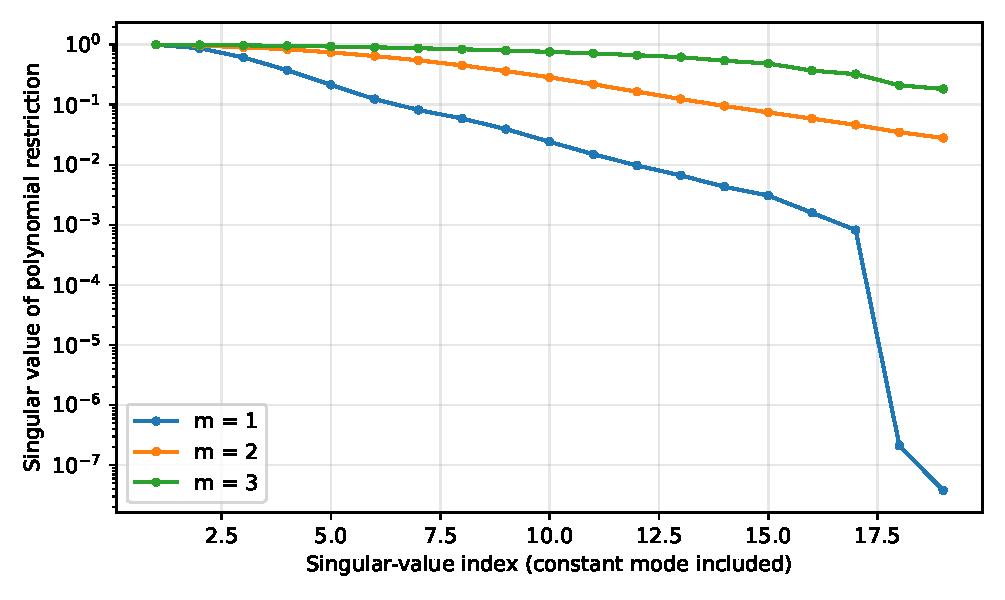
\includegraphics[width=.94\linewidth]{figures/polynomial_spectra.pdf}
\caption{Finite polynomial singular values for $q=1/2$, degrees $0$ through $18$. These are singular values of restrictions, not exact values of the infinite spectrum. The small values at the end of a finite list may approximate null directions, as explained after \cref{thm:factorial}.}
\label{fig:spectra}
\end{figure}

\subsection{Certified algebraic quantities versus rounded diagnostics}
The exact fraction
\begin{equation}
 T_N=\norm{C_N}_\HS^2
 =\sum_{j=0}^{N}\norm{\calC e_j^X}_2^2
 \label{eq:trace-lower}
\end{equation}
is also produced. It is nondecreasing in $N$ and converges to $e^{I_2}$, by Parseval and the Hilbert--Schmidt theorem. Thus $\log T_N$ is a genuine analytic lower bound for $I_2$; the CSV retains the exact numerator and denominator of $T_N$. A decimal rendering of its logarithm is not an interval certificate. Likewise, finite polynomial centered norms increase to $\rho_*$, because polynomials are dense and conditional expectation is bounded. The numerical eigenvalues are not presented as verified interval enclosures.

To reproduce the package, run
\begin{verbatim}
python -m pip install -r requirements.txt
python verify.py --degree 18
latexmk -pdf -interaction=nonstopmode -halt-on-error article.tex
\end{verbatim}
The program rejects invalid $q$, depth, and diagnostic-degree choices. The final PDF does not need Python to rebuild when the included table and figure are retained.

\section{Consequences for the repository's open questions}
\label{sec:answers}
\subsection{The Bayesian spectral question}
The operator is now triangularized algebraically in monomials and intertwined in its natural Appell families. Its complete finite Jordan type is given, but that is deliberately separated from the weighted singular problem. Every finite singular invariant is an exact moment-matrix expression, including all exterior powers. The suggested $q^{mn}$ diagonal is not correct for the defined operator: the monic polynomial diagonal is one, and the degree-one Hilbert coefficient is $\sqrt{1-q^{2m}}$.

% ed. (2026-09-29): the refuted expectation is now marked incorrect in the source report.
\begin{ednote}
The source report now carries an editorial note, directly after
\texttt{prob:Bayesian-spectrum} in
\path{inverse-and-sampling/fabius_information_frontier/fabius_information_frontier.tex},
that marks its expected $q^{mn}$ Appell diagonal incorrect for the operator
it defines and points to this article (Proposition~\ref{prop:appell}); the report's
README records the same erratum.
\end{ednote}

The infinite operator is compact of every Schatten order, has dense range, and loses an infinite-dimensional explicit family of Fourier modes. A degree-ordered orthogonal polynomial diagonalization is excluded by the nonzero cubic coefficient, and more generally by Gaussian rigidity. The complete positive singular sequence has not been expressed in closed form. Neither the all-Schatten result nor the existence of a singular decomposition should be mistaken for such a formula.

\subsection{The R\'enyi question}
The finite-depth integrals exist for every finite order, including every positive integer. Collision information has the exact trace representation \eqref{eq:collision-trace}, explicit two-sided bounds, monotone moment-computable lower bounds, and the critical asymptotic \eqref{eq:collision-limit}. A finite limiting excess exists precisely through order two among the orders $\alpha>1$. This supplies a structural answer that the earlier formal Thue--Morse integral alone did not give. A closed finite multi-sum for every integer order is not asserted.

\subsection{The corrected-prefix rate-distortion question}
The exact distortion identity excludes the entire class of prefix-only corrections, even randomized ones, at $D_m$. A separate Gaussian observation test channel is strictly better for every depth, not only asymptotically. The remaining rate-distortion expansion is a different problem and is not silently declared solved.

\section{Further research questions and proposed routes}
\label{sec:future}
\begin{problem}[Sharp positive singular-value asymptotics]
Determine the actual asymptotic size of $s_n(\calC)$. Is the coefficient $1/[6\log(1/q)]$ in the upper bound improvable, and what is the correct scale? The factor three in the proof comes from grouping three uniforms per derivative, not from an optimality argument. A sharper weighted derivative factorization or a lower bound based on localized test functions would be informative.
\end{problem}

\begin{problem}[Complete nullspace synthesis]
Does the closed span of the exponential-polynomial modes from all zeros of $\phi_T$ equal $\ker\calC$? The present theorem only constructs a subspace. This is a finite-interval convolution equation with weighted norms, so a spectral-synthesis theorem must be checked in precisely that setting rather than borrowed formally from a whole-line transform calculation.
\end{problem}

\begin{problem}[Growth above the critical R\'enyi order]
For fixed $\alpha>2$, determine the sharp growth of $I_\alpha-R_m$. The proof here establishes divergence but no rate. Endpoint saddle-point estimates suggest that the competition between the moving prefix endpoint and the log-normal small-tail scale should matter. A useful first target is to determine whether growth is quadratic in $m$ and to establish matching upper and lower bounds before proposing an all-orders expansion.
\end{problem}

\begin{problem}[Critical crossover]
Study $\alpha=2+u/m$ or other joint scalings as $m\to\infty$. Fixed-order dominated convergence stops exactly at two, whereas each finite-depth function is finite at larger orders. The transition region is therefore a natural place for a uniform asymptotic analysis, potentially involving the endpoint inverse-Fabius expansions already present in the repository.
\end{problem}

\begin{problem}[Certified collision-information evaluation]
Combine the exact rational traces $T_N$ with certified bounds on the complementary Hilbert--Schmidt tail. The output-Jacobi approximation in \eqref{eq:finite-rank-bound} gives a separate explicit route to finite-rank enclosures. A practical implementation should avoid confusing output projections with input moment truncations and should use interval eigenvalue bounds, rather than rounded high-precision numbers, for final certificates.
\end{problem}

\begin{problem}[Rate-distortion beyond the Shannon lower bound]
Find the first nonzero correction, or prove that all algebraic corrections vanish, in $R_X(D)$ as $D\downarrow0$ for the flat geometric-uniform density. The prefix-only route is now excluded at its exact distortion. A corrected backward Gaussian channel or a controlled reverse-heat construction would have to address positivity and the moving compact boundary explicitly.
\end{problem}

\begin{problem}[Maximum correlation and optimal nonlinear statistics]
Determine $\rho_*(S_{q,m},X_q)$, or give efficient certified enclosures. The cubic witness proves a strict nonlinear advantage, but the degree-18 values are only lower approximations. The two-variable parity blocks, exact moment pencils, and dense-range theorem give a concrete starting point for a convergent scheme.
\end{problem}

\begin{problem}[Formalization and general masks]
Formalize the algebraic finite-matrix results first: moment recurrences, Appell intertwining, Jordan ranks, the determinant ratio, and the cubic obstruction. Then isolate the analytic kernel estimate and weighted Jacobi approximation as reusable lemmas. For other innovation masks, identify conditions replacing finite-uniform endpoint geometry and triple-factor Fisher bounds. No equality of ordinary polynomial eigenvalues and Hilbert singular values should be built into the interface.
\end{problem}

\section{Provenance, validation boundary, and conclusion}
\label{sec:provenance}
The repository navigation was inspected on 29 September 2026. The recursive tree response reported snapshot
\begin{center}\small\texttt{8490a6e1c259a3b0c7ce32170816740b8ad7b40d}.\end{center}
The current inverse-and-sampling README was used to identify the information-frontier package and distinguish it from the recent entropy-Edgeworth and uniform-factor-recovery intakes. Detailed question wording was read from the user's Library copy of \path{fabius_information_frontier.tex}, dated 30 August 2026. That materialized copy has 77,282 bytes and SHA-256
\begin{center}\scriptsize\texttt{b756c86255c24f421029ded2f60f574f0677fbad4bb0fa62416950a742ebda45}.\end{center}
The live repository metadata described a different, 78,310-byte source. Accordingly, this article does \emph{not} claim byte-identical correspondence between the Library copy and the current repository article. The mathematical definitions and source labels used above are stated explicitly so that the results can be checked independently of editorial changes. No existing repository proof, formally verified or otherwise, is an unexamined assumption in the principal analytic arguments.

% ed. (2026-09-29): provenance identified on filing (no hashes added).
\begin{ednote}
The hexadecimal string above identifies a repository commit, not a tree
object; the source report at that commit is identical to the current one.
The Library copy is byte-identical to the source report as first archived in
the repository on 30 August 2026. Between that version and the current
78,310-byte file, the three source problems cited here changed only by
renamings of notation macros, so the wording used above is, mathematically,
that of the current report.
\end{ednote}

The supplied script was executed with degree eighteen and 100-digit numerical arithmetic after the exact fraction computations. Its report separates exact checks from numerical diagnostics. The PDF was compiled from the included source and visually checked after rendering. There is no Lean file, no claim of kernel certification, and no assertion that a literature-wide novelty search is exhaustive.

The central lesson is a precise one. Conditional expectation can be perfectly invertible in each finite polynomial coefficient space while having infinitely many exact null modes after Hilbert completion. Its nonzero spectrum can be extremely small while its likelihood ratio remains unbounded. And every finite R\'enyi order can exist at every depth while a sharp critical order appears in the depth limit. The geometric-uniform channel makes all three distinctions explicit and provable.

\begin{thebibliography}{9}
\bibitem{repo}
V.~Reshetnikov, \emph{ProveIt}, GitHub repository, inspected 29 September 2026. In particular, the FabiusFunction inverse-and-sampling research-frontier navigation.
\url{https://github.com/VladimirReshetnikov/ProveIt}.

\bibitem{frontier}
\emph{Exact Information Geometry and New Frontiers for the Fabius Function, Rvachev's Up-Function, Thue--Morse Sinc Products, and Geometric $q$-Convolutions}, research report prepared for Vladimir Reshetnikov, 30 August 2026. Source file \path{fabius_information_frontier.tex}; question labels \texttt{prob:Bayesian-spectrum}, \texttt{prob:TM-Renyi}, and \texttt{prob:exact-RD}. The Library-copy provenance is recorded in \cref{sec:provenance}.

\bibitem{arias}
J.~Arias de Reyna, \emph{An infinitely differentiable function with compact support: Definition and properties}, English translation of the 1982 paper, arXiv:1702.05442, 2017.
\url{https://arxiv.org/abs/1702.05442}.

\bibitem{anshelevich}
M.~Anshelevich, \emph{Appell polynomials and their relatives}, International Mathematics Research Notices 2004, no.~65, 3469--3531; arXiv:math/0311043v3.
\url{https://arxiv.org/abs/math/0311043}.

\bibitem{dlmf}
NIST, \emph{Digital Library of Mathematical Functions}, Chapter 18, especially \S18.9, Jacobi derivative identities; accessed 29 September 2026.
\url{https://dlmf.nist.gov/18.9}.

\bibitem{xu}
Y.~Xu, \emph{Approximation by polynomials in Sobolev spaces with Jacobi weight}, arXiv:1608.04114, 2016.
\url{https://arxiv.org/abs/1608.04114}.

\bibitem{anantharam}
V.~Anantharam, A.~Gohari, S.~Kamath, and C.~Nair, \emph{On maximal correlation, hypercontractivity, and the data processing inequality studied by Erkip and Cover}, arXiv:1304.6133, 2013.
\url{https://arxiv.org/abs/1304.6133}.

\bibitem{renyi}
T.~van Erven and P.~Harremo\"es, \emph{R\'enyi divergence and Kullback--Leibler divergence}, arXiv:1206.2459, 2012; IEEE Transactions on Information Theory 60 (2014), 3797--3820.
\url{https://arxiv.org/abs/1206.2459}.

\bibitem{koch}
T.~Koch, \emph{The Shannon lower bound is asymptotically tight}, arXiv:1504.08245, 2015.
\url{https://arxiv.org/abs/1504.08245}.
\end{thebibliography}
\end{document}
